\chapter{TIDLIGERE - Problemanalyse}
\textit{I dette kapitel analyses problemstillinger, som opstår i forbindelse med lægemiddelskift. Disse problemstillinger vil sammenfattes i en opsummering og afsluttes med en problemformulering, der fremadrettet danner  grundlaget for rapporten.}

\section{Årsager til lægemiddelskift}
Lægemiddelskift kan forekomme i forbindelse med kontraktskift, bagatelkøb eller restordre~\citep{Amgros2015}. Kontraktskift kan forekomme ved at lægemidlerne sendes i udbud, såkaldt amgrosudbud. Udbuddene forekommer hvis der findes mere end én leverandør af lægemidlet. Lægemidlerne bringes derved i konkurrence, hvilket kan give anledning til kontraktskift. I tilfælde af patent på lægemidlet, hvormed der kun findes én leverandør, er der ofte ikke konkurrence, da prisen på lægemidlet allerede er fastsat.~\citep{Amgros2015} 

En gang årligt omkring maj eller juni publiceres bagatelkøb af Amgros, hvilket kan forårsage lægemiddelskift~\citep{Amgros2018}. I disse tilfælde modtager Amgros pristilbud fra leverandørere med henblik på økonomiske besparelser på lægemiddlerne~\citep{Amgros2012}. I disse tilfælde er Sygehusapoteket er ikke forpligtet til at anvende lægemidlet og leverandøren omfattes ikke af indkøbs- eller forsyningspligt, som ved kontraktskift.~\citep{Amgros2018}

Restordre forekommer når efterspørgslen på et lægemiddel overstiger den tilgængelige mængde.~\citep{Amgros2015}. Dette kan f.eks. ske ved leveringesvigt fra leverandøren eller producenten på det ønskede lægemiddel~\citep{Amgros2017, Laegemiddelinformaion2017}. Leveringesvigt skyldes som ofte at producenten har mangel på råvarer eller produktionsvanskeligheder~\citep{Amgros2017, Laegemiddelinformaion2017}. I tilfælde  af restordre er det leverandørens ansvar at dække hospitalsapotekernes udgift ved indkøb af et erstatningslægemiddel\fxnote{KILDE}.

\section{Lægemiddeludbud}
Størstedelen af udbud på lægemidler i ATC-grupper sker en gang årligt fra start september til midt november, hvor udbud på ATC-grupper som indgår i RADS behandlingsvejledninger \fxnote{\url{http://www.rads.dk/behandlingsvejledninger}} sker løbende hen over året.~\citep{Sygehusapoteket2017}

Et udbud kan ske ved to udbudsformer, som er defineret på forhånd, enten på baggrund af lægemidlets pris, hvilket er tilfældet for de fleste lægemidler, eller ved økonomisk mest fordelagtige udbud, hvor prisen vægtes mod andre kriterier ~\citep{Amgros2018a}. Disse kriterier er opstillet på baggrund af juridiske grundlag og kan f.eks. omfatte emballage, håndtering af lægemidlet ved administration samt patientsikkerhedsmæssige aspekter. Der kan være én eller flere vindere ved hver udbudsform, hvilket medfører fire typer af udbud.~\citep{Amgros2018a} De fire udbudstyper fremgår af figur \ref{fig:TypeUdbud}.

\begin{figure}[H]\centering
	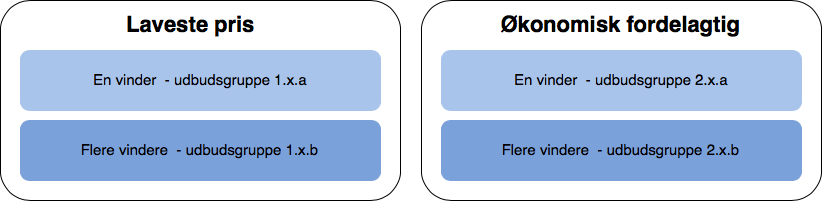
\includegraphics[width=0.7\textwidth]{billeder/TypeUdbud.png} 
	\caption{Udbudstyper herunder laveste pris og økonomisk fordelagtig. De to udbudstyper er opdelt i fire typer udbud, hvor grupper med 1 vinder er angivet med 1 og flere vinder er angivet med 2. Bogstaverne a og b angiver henholdsvis om der er tale om en rammeaftale eller flere parallelle rammeaftaler. ~\citep{Amgros2018a}}
	\label{fig:TypeUdbud}  
\end{figure}

Når et udbud sker indsender ansøgende leverandører en omkostnings- og budgetkonsekvensanalyse for nye lægemidler og indikationer til Medicinrådet~\citep{Amgros2017, Amgros2017a}. Omkostningsanalysen omfatter samfundsomkostninger per patient for den nuværende og den ansøgte behandling.
Budgetkonsekvensanalysen omhandler de samlede økonomiske konsekvenser for regionerne ved at anvende det ansøgte lægemiddel.~\citep{Amgros2017a}

Analyserne vurderes på vegne af Medicinrådet af Amgros i forhold til relevans og valide oplysninger.~\citep{Amgros2017, Amgros2017a} Der vurderes, relevans i klinisk praksis, overholdelse af metodevejledning, kvalitet af omkostningsmodellen og overordnede usikkerheder samt evidensens kvalitet. Yderligere kategoriseres de nye lægemidler og indikationer i forhold til den nuværende behandling i stor, vigtig, lille eller ingen merværdi af Medicinrådet.~\citep{Amgros2017, Amgros2017a}

Den kliniske merværdi og analyserne danner grundlaget for prisforhandling~\citep{Amgros2017, Amgros2017a}. Amgros forhandler med den ansøgende leverandør for at opnå retfærdigt forhold mellem merværdi og meromkostninger i forhold til den nuværende og ansøgte behandling. Ud fra beslutningsgrundlag på forhandlingerne udarbejder Amgros en anbefaling til Medicinrådet.~\citep{Amgros2017, Amgros2017a}

På baggrund af den indsamlede evidens og resultatet af forhandlingerne foretaget af Amgros beslutter Medicinrådet hvorvidt lægemidlet skal anvendes som standardbehandling.~\citep{Amgros2017a} 

\section{Indkøb af lægemidler}
Indkøb af lægemidler til distribution til de nordjyske hospitaler foretages af Sygehusapoteket Region Nordjylland (SRN)~\citep{SygehusapoteketRegionNordjylland2013}. Salg til Region Nordjyllands (RN) egne institutioner udgør 98,4~\% af det samlede salg i år 2012, hvor under 1~\% går til andre regioners sygehusapoteker og til private apoteker samt andre kunder. Udover indkøb yder SRN information og tilbyder tjenesteydelser til de kliniske afsnit, herunder klinisk farmaci.~\citep{SygehusapoteketRegionNordjylland2013}

Størstedelen af medicinindkøb i år 2012, svarende til 95~\%, skete via. Amgros. Yderligere blev 2~\% købt af andre sygehusapoteker, 1~\% fra private apoteker og 2~\% fra øvrige. ~\citep{SygehusapoteketRegionNordjylland2013}
Bestilling af medicin fra hospitalsafsnittene sker via medicinservice varetaget af farmakonomer. Der bestilles medicin via ApoVision-Online. SRN forgår som lagerholder og fremtager medicin manuelt fra henholdsvis almindeligt hyldelager, pater Noster (halvautomatik lager-reol) og høj-lager (paller).~\citep{SygehusapoteketRegionNordjylland2013}

SRN er opdelt i forskellige afdelinger herunder ledelse, administration, lægemiddelinformation, klinisk farmaci, logistik, kvalitetsafdeling og produktion. De primære aktører ved Amgrosudbud i RN er Amgros-ansvalige, Specialistfarmaceut/ATC-asnarlige og Lægemiddelinformation. Opgaver for disse aktører fremgår af figur\ref{fig:SRNudbud}.

\begin{figure}[H]\centering
	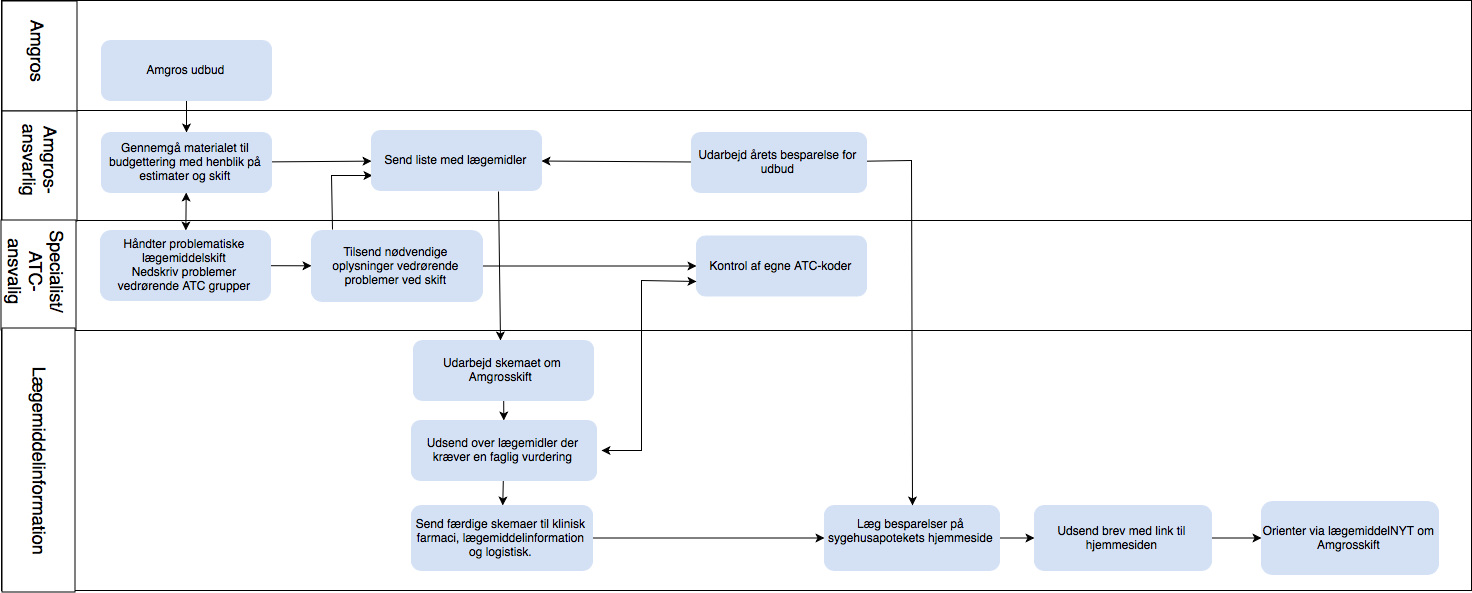
\includegraphics[width=1\textwidth]{billeder/SRNudbud.png} 
	\caption{...}
	\label{fig:SRNudbud}  
\end{figure}

Ved Amgrosudbud står den Amgros-ansvalige  for at gennemgå udbudsmaterialet og budgettestimere i forbindelse med kommende kontrakter. I sammenhæng med dette håndteres problematiske lægemiddelskift af specialist/ATC-ansvarlige. De problemer der vedrører ATC-grupper nedskrives og sendes tilbage til den Amgros-ansvarlige. Den Amgros-ansvarlige sender herefter en liste ud med lægemidler til Lægemiddelinformation, hvorefter der udarbejdes et skema om lægemiddelskift. Lægemiddelinformation udsender herefter en liste med lægemidler der kræver en faglig vurdering til Specialistfarmaceut/ATC-asnarlige, som kontrollere egne ATC-koder. Herefter sendes færdige skemaer til Klinisk farmaci, Lægemiddelinformationen og Logistik i SRN. Dernæst udarbejdes årets samlede besparelse af Amgros-ansvarlige og ligges på Sygehusapotekets hjemmeside af Lægemiddelinformationen som også sender brev med link til hjemmesiden og orientere via LægemiddelNyt omkring Amgrosskift. 

\section{Implementering af lægemiddelskift}
Implementering af lægemiddel kategoriseres efter sværhedsgrader som simpel eller kompleks på baggrund af flere faktorer som f.eks. hvem skiftet har betydningen for, om der er nogle begrænsninger for hvornår et skift kan finde sted og risikovurdering af hvordan det påvirker afsnittet~\citep{Sygehusapoteket2017b}.

Et simpelt lægemiddelskift er vurderet til at påvirke klinikken i lav grad og varetages ofte af logistik-afdeling, hvorimod et kompleks lægemiddelskift påvirker klinikken i mellem til høj grad, hvorfor flere interessenter involveres ved disse skift.~\citep{Laegemiddelinformaion2017,Sygehusapoteket2017a}. 

Simple lægemiddelskift sker til dagligt i forbindelse med at et lægemiddel skiftes, på grund af restordre, til et simpel generisk lægemiddel~\citep{Laegemiddelinformaion2017}. De komplekse skift sker i forbindelse med ændringer af generiske lægemidler som f.eks. styrke, disponeringsform og ændring i hjælpestoffer. Ofte kontaktes interessenter som medicinansvarlige, kontraktsygeplejersker eller medicinservicefarmakonomerne i forhold til at undersøge lægemidlets anvendelighed for det pågældende hospitalsafsnit.~\citep{Laegemiddelinformaion2017,Sygehusapoteket2017a}

\section{Problemstillinger ved lægemiddelskift}
I forbindelse med lægemiddelskift kan der opstå utilsigtede hændelser (UTH'er)~\citep{Amgros2015}. De hyppigste årsager til UTH'er på de danske hospitaler skyldes i år 2013 medicinering, hvilket udgjorde 23,97~\%.~\citep{Patientombuddet2013}. Antallet af rapporterede UTH'er i Region Nordjylland er steget med over 36\% fra år 2012 til 2014 ~\citep{Jensen2014}. Ud af 824 rapporterede UTH'er i år 2014 omhandlede 97\% medicinering, 86\% administration af medicin og 41\% disponering~\citep{Jensen2014}. Det er i flere studier undersøgt de utilsigtede hændelser forårsaget af henholdsvis ordinationer, dispensering og administration af medicin, hvilket fremgår af tabel \ref{table:UTHordination}, \ref{table:UTHdispensering} og \ref{table:UTHAdministration}. En fælles årsag til rapporterede UTH'er er forkert dosis, forkert lægemiddel og udeladelse af henholdsvis ordination, dispensering og administration.

	\vspace{2mm}
\begin{longtable}{p{5.5cm}|p{3cm}|p{2cm}|p{2.3cm}}
	\caption{Utilsigtede hændelser ved ordinationer.}
	\vspace{2mm}
	\label{table:UTHordination} \\
\cellcolor[HTML]{C0C0C0} {\textbf{Årsager}} & 
{\cellcolor[HTML]{C0C0C0}\textbf{Sundhedsstyrelsen~\citep{Sundhedsstyrelsen2005}}} &
{\cellcolor[HTML]{C0C0C0}\textbf{Lisby et al~\citep{Lisby2005}}} &
{\cellcolor[HTML]{C0C0C0}\textbf{Tully et al~\citep{Tully2009}}} \\ \hline
%{\cellcolor[HTML]{C0C0C0}\textbf{4}} 
%\textbf{Metode} & Gennemgang af indberettede UTH'er & Observation, stikprøvekontrol, journalgennemgang & Gennemgang af medicinlister & Gennemgang af indberettede UTH'er \\ \hline
Forkert dosis & - & - & 12,5~\%  \\ \hline %& 29,6      \\ \hline
Forkert lægemiddel & 16,3~\% & - & - \\ \hline % & 14,5 \\ \hline
Forkert patient & 3,8~\% & - & - \\ \hline %& 11,2 \\ \hline
Intet lægemiddel ordineret & 20,7~\% & - & 15,9~\% \\ \hline % & 24,1 \\ \hline
Udeladelse af formulering & - & 38,0~\% & - \\ \hline %& - \\ \hline
Udeladelse af administrationsvej & - & 34,7~\% & - \\ \hline %& - \\ \hline
Udeladelse af doseringstidspunkt & - & 10~\% & 10,4*~\% \\ \hline %& - \\ \hline
Manglende angivelse af maskimal dosis & - & - & 12,1~\% \\ \hline %& -  \\ \hline
Overset kontraindikation & 14,3~\% & - & 0,3~\% \\ \hline %& 19,6 \\ \hline
\cellcolor[HTML]{C0C0C0} {\textbf{Total antal fejl}} & 
{\cellcolor[HTML]{C0C0C0}\textbf{526}} &
{\cellcolor[HTML]{C0C0C0}\textbf{320}} &
{\cellcolor[HTML]{C0C0C0}\textbf{3455}}
\end{longtable}

Ud fra tabel \ref{table:UTHordination} fremgår det at de hyppigste årsager til UTH ved ordinationer skyldes 38~\% af de 320 rapportede UTH'er udeladelse af formulering og 34,7~\% administrationsvej~\citep{Lisby2005}. To studier påviste at i 20,7~\% ud af 526 og 15,9~\% af 3455 skyldes at intet lægemiddel var ordineret~\citep{Sundhedsstyrelsen2005, Tully2009}. Årsager som intet lægemiddel ordnineret, udeladelse af doseringstidspunkt samt overset kontraindikation er dokumenteret af flere studier~\citep{Sundhedsstyrelsen2005, Lisby2005, Tully2009}. 

\vspace{2mm}
\begin{longtable}{p{5cm}|p{3.5cm}|p{2cm}|p{2.3cm}}
	\caption{Utilsigtede hændelser ved dispensering.}
	\vspace{2mm}
	\label{table:UTHdispensering} \\
\cellcolor[HTML]{C0C0C0} {\textbf{Årsager}} & 
{\cellcolor[HTML]{C0C0C0}\textbf{Sundhedsstyrelsen~\citep{Sundhedsstyrelsen2005}}} &
{\cellcolor[HTML]{C0C0C0}\textbf{Lisby et al~\citep{Lisby2005}}} &
{\cellcolor[HTML]{C0C0C0}\textbf{Barker et al~\citep{Barker2002}}} \\ \hline
%\textbf{Metode} & Gennemgang af indberettede UTH'er & Observation, stikprøvekontrol, journalgennemgang & Gennemgang af medicinlister & Gennemgang af indberettede UTH'er \\ \hline
Forkert dosis & 26,6~\% & 29,4~\% &  20,0~\% \\ \hline
Forkert lægemiddel & 52,2~\% & - & - \\ \hline
Forkert tidspunkt & - & 1,1~\% & 40,3~\% \\ \hline
Udeladt dispensering & 11,4~\% & 41,2~\% & 27,9~\% \\ \hline
%Dispensering af et
Ikke ordineret lægemiddel & - & 29,4 & 4,8 \\ \hline
\cellcolor[HTML]{C0C0C0} {\textbf{Total antal fejl}} & 
{\cellcolor[HTML]{C0C0C0}\textbf{184}} &
{\cellcolor[HTML]{C0C0C0}\textbf{17}} &
{\cellcolor[HTML]{C0C0C0}\textbf{290}}
\end{longtable}

Ud fra tabel \ref{table:UTHdispensering} fremgår det at de hyppigste årsager til UTH ved dispensering skyldes i 52,2~\% af de 184 rapporterede UTH'er forkert lægemiddel. Udover forkert lægemiddel blev der påvist forkert dosis, forkert tidspunkt eller udeladelse af dispensering samt ikke ordineret lægemiddel, hvor årsagerne er dokumenteret i flere af studierne~\citep{Lisby2005, Sundhedsstyrelsen2005,Barker2002}.

\vspace{2mm}
\begin{longtable}{p{5.5cm}|p{3.5cm}|p{2cm}|p{2.3cm}}
	\caption{Utilsigtede hændelser ved administration.}
	\vspace{2mm}
	\label{table:UTHAdministration} \\
\cellcolor[HTML]{C0C0C0} {\textbf{Årsager}} & 
{\cellcolor[HTML]{C0C0C0}\textbf{Sundhedsstyrelsen~\citep{Sundhedsstyrelsen2005}}} &
{\cellcolor[HTML]{C0C0C0}\textbf{Lisby et al~\citep{Lisby2005}}} &
{\cellcolor[HTML]{C0C0C0}\textbf{Barker et al~\citep{Barker2002}}} \\ \hline
%\textbf{Metode} & Gennemgang af indberettede UTH'er & Observation, stikprøvekontrol, journalgennemgang & Gennemgang af medicinlister & Gennemgang af indberettede UTH'er \\ \hline
Forkert dosis & 37,5~\% & - & 20,0~\% \\ \hline
Forkert lægemiddel & 19,1~\% & - & - \\ \hline
Forkert tidspunkt & 8,9~\% & - & 40,3~\% \\ \hline
Forkert patient & - & 15,7~\% &  - \\ \hline
Udeladt administration & 15,0~\% & - & 27,9~\% \\ \hline
Manglende patientidentifikation & - & 78,9~\% & - \\ \hline
\cellcolor[HTML]{C0C0C0} {\textbf{Total antal fejl}} & 
{\cellcolor[HTML]{C0C0C0}\textbf{839}} &
{\cellcolor[HTML]{C0C0C0}\textbf{190}} &
{\cellcolor[HTML]{C0C0C0}\textbf{290}}
\end{longtable}
\vspace{0.25cm}

Ud fra tabel \ref{table:UTHAdministration} fremgår det at de hyppigste årsager til UTH ved administration i 78,9~\% af de 190 rapporterede UTH'er manglende patientidentifikation~\citep{Lisby2005}. I et af studierne skyldes 40,3~\% ud af 290 af tilfældene forkert tidspunkt~\citep{Barker2002} og i 37,5~\% af 839 forkert dosis~\citep{Sundhedsstyrelsen2005}. Forket dosis, forkert tidspunkt og udeladt administration var dokumenteret i flere studier~\citep{Lisby2005,Sundhedsstyrelsen2005,Barker2002}.

\subsection{Utilsigtede hændelser ved kontraktskift}
De patientsikkerhedsmæssige konsekvenser opstået ved kontraktskift er undersøgt af et norsk studie~\citep{Hakonsen2010}. Interview med 100 sygeplejersker påviste at der opstod fejlmedicinering ved generiske lægemidler. Fejl i ordination og manglende dokumentation af lægemiddelskiftet foretaget af lægen blev opdaget af 46~\% sygeplejersker dagligt, hvorimod sygeplejerskerne altid fik lægemiddelsiftet dokumenteret. Yderligere følte 92~\% af sygeplejerskerne at generiske lægemidler var tidskrævende og 91~\% at disse øgede risikoen for fejl ved disponering.~\citep{Hakonsen2010}. De typiske hændelser ved kontraktskift fremgår af Figur \ref{fig:UTHkontraktskift}.

\begin{figure}[H]\centering
	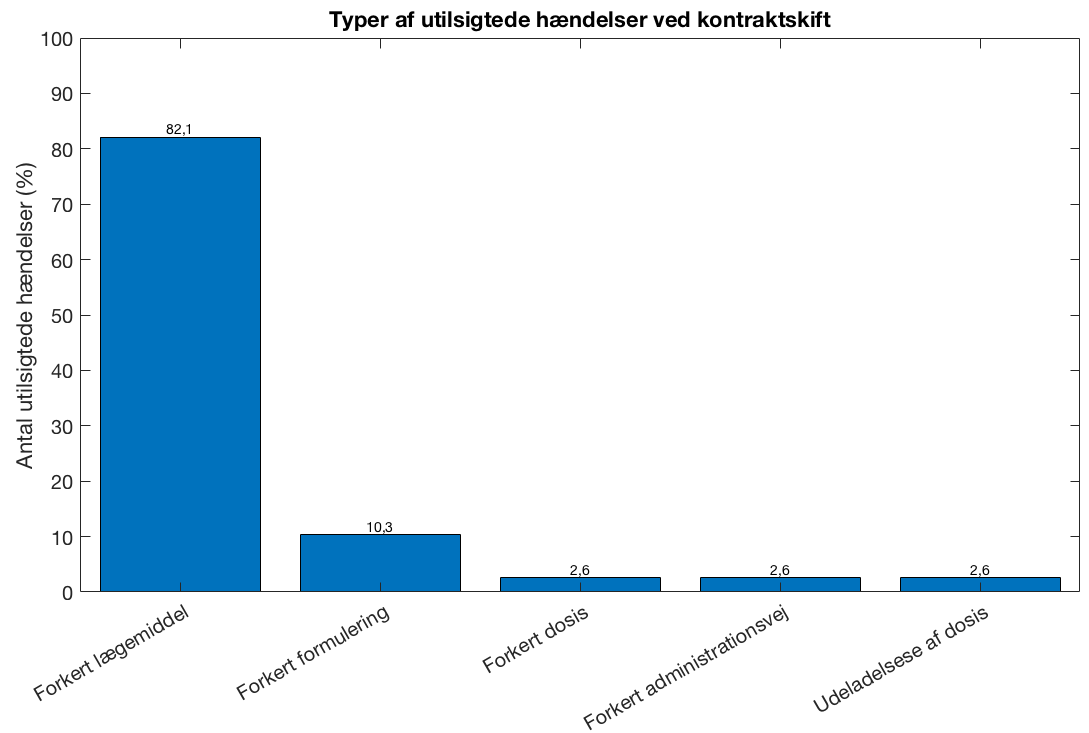
\includegraphics[width=1\textwidth]{billeder/UTH1.png} 
	\caption{Utilsigtede hændelser opstået ved kontraktskift\citep{Hakonsen2010}.}
	\label{fig:UTHkontraktskift}  
\end{figure}

Af Figur \ref{fig:UTHkontraktskift} fremgår det at 82,1~\% af UTH'erne forekommer ved disponering af forkert lægemiddel. Den næst hyppigste er forkert formulering hvor 10,3\% af UTH'er er berettiget mod dette. I  sjældnere tilfælde sker forkert dosis, administrationsvej samt udeladelse af dosis. 

\subsection{Utilsigtede hændelser ved restordre}
Studie har påvist at restordre påvirker patientsikkerheden ved anvendelse af generisk lægemiddel eller manglende alternativ behandling~\citep{Baumer2004}. Gennem spørgeskemaundersøgelse besvaret af farmaceuter blev UTH'er identificeret ved restordre. Undersøgelsen skelner mellem opståede hændelser og nærhændelser, som kunne være opstået~\citep{McLaughlin2013,McBride2013}. Typer af UTH'er identificeret ved restordre fremgår af figur \ref{fig:UTHrestordre}. 


\begin{figure}[H]\centering
	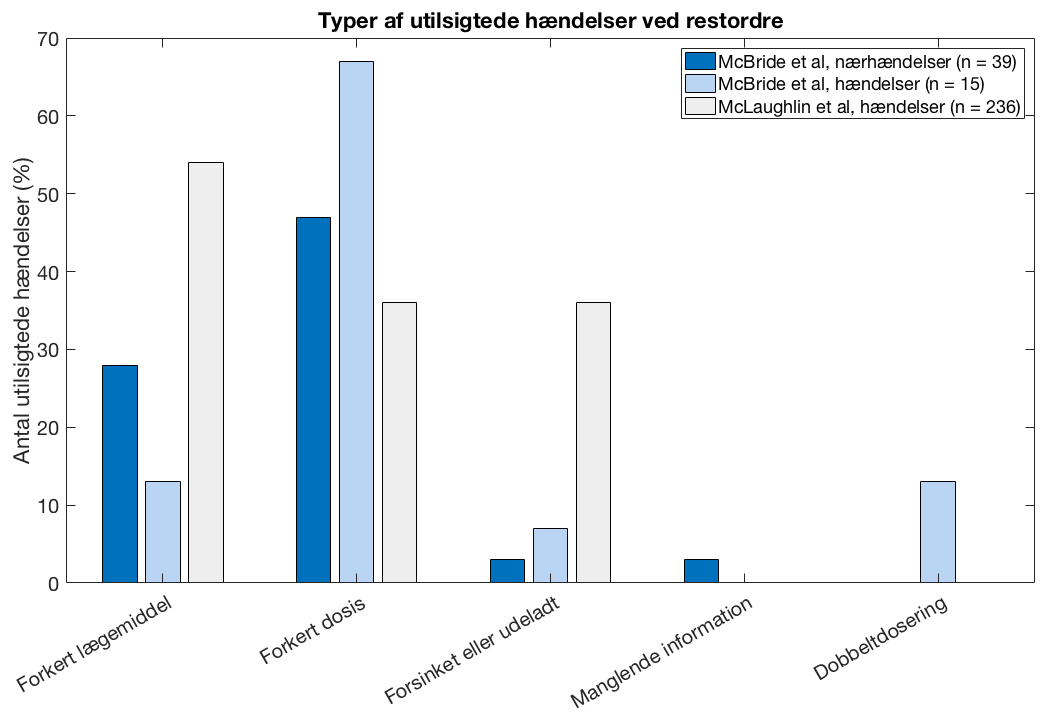
\includegraphics[width=1\textwidth]{billeder/UTH2.png} 
	\caption{Utilsigtede hændelser opstået ved restordre~\citep{McLaughlin2013,McBride2013}.}
	\label{fig:UTHrestordre}  
\end{figure}

Ud fra figur \ref{fig:UTHrestordre} fremgår det at forket dosis af lægemiddel og forsinket dosis var den hyppigste type af UTH ved restordre~\citep{McLaughlin2013,McBride2013}. Yderligere blev der i studierne identificeret UTH ved forsinket eller udeladt af dispensering og administrering. Manglende information og dobbeltdosering blev påvist i et af studierne som en årsag til UTH ved restordre.~\citep{McLaughlin2013,McBride2013}

\section{Forebyggelse af utilsigtede hændelser}
De hyppigeste utilsigtede hændelser opstår i forbindelse med medicinering, administration og disponering~\citep{Jensen2014}. 
En måde at begrænse antallet af UTH'er er at synliggøre de problemstillinger der har medført til en UTH. Ved at rapportere UTH'er kan de bagvedliggende årsager til fejl forebygges. Indbretningen af UTH'er er for sundhedsprofesionelle lovpligtigt~\citep{Jensen2014}. Yderligere blev det i år 2011 muligt for pårørende at rapportere UTH'er~\citep{Jensen2014}. På baggrund af rapporterede UTH'er er forskellige metoder anvendt til at løse nogle af de problematikker der opstår.

\subsection{Elektronisk patientmedicinering}
Studier har påvist at implementering af elektronisk beslutningsstøtte reducerer antallet af UTH'er~\citep{DW1998,Bates2013,Cheng2011,Raboel2005} og beskrives som et vigtigt redskab til at øge kvaliteten af medicinering med henblik på at nedbringe fejl~\citep{Raboel2005}. I Danmark har indførsel af elektronisk patientmedicinering (EPM) medvirket til at reducere antallet af medicineringsfejl. Dette hjælper med at simplificere selve medicineringsprocessen, da dokumentation af ordination, dispensering og administration er samlet i ét system. Dette hjælpemiddel anvendes som et passivt beslutningsstøte for lægen ved ordination.
Medicineringsfejl kan yderligere nedsættes hvis der udnyttes aktiv elektronisk beslutningsstøtte, hvor lægen vejledes f.eks. i forhold til lægemiddeldosis eller advares, hvis ordination kan være skadelig for patienten.~\citep{Raboel2005}. 

På trods af at EPM har påvist at reducere antallet af UTH'er ved medicinering er der rapporteret UTH'er ved anvendelse af EPM~\citep{Syddanmark2008}, hvorfor der bør være fokus på forbedring og anvendelse af teknologier. 

%- Ny it-platform letter arbejdsgangene APOTO. APOTO skal levere data af høj kvalitet om lægemidler til sygehusenes EPJ systemer og på længere sigt kansystemet udvikles til også at under-støtte sygehusapotekernes produktion af lægemidler.  %[KILDE:Amgros_Årsmagasin2014, side 12]

\subsection{Stregkode scanning}
Internationale studier har påvist at stregkode scanning af lægemidler har en effekt på reducering af fejl i medicineringsprocessen~\citep{Poon2006,Bates2000,Levtzion-korach2010}. I Danmark anvender størstedelen af hospitalerne stregkode scanning, hvor lægemidlet kan spores fra leverandøren til patienten, hvilket medvirker til en effektiv lægemiddelforsyning og sikker medicinering ~\citep{Dzik2007,DPSD2008,Amgros2013}. Amgros har siden år 2010 stillet krav til stregkode på yderste og inderste emballage på lægemidler~\citep{Amgros2013}. Foruden at undgå alvorlige medicinrelaterede hændelser og reducere omkostninger samt tidsforbruget ved lagerstyring kan stregkoder også medfører andre positive resultater såsom, sikre registering af lægemiddel i patienternes medicinjournal og effektiv tilbagekaldelse af medicin via it-systemer~\citep{Amgros2013}.
Implementering af stregkode scanning er påvirket af manglende stregkoder og dokumentation ved generisk lægemiddel. 

\subsection{Klar-til-brug lægemidler}
Internationale studier har påvist at automatisk dosisdispensering reducerer antallet af medicineringsfejl~\citep{Oren2003,Sygehusapotekerne2012}. I Danmark er der endnu ikke dokumenteret effekt på medicineringsfejl ved automatisk dosisdispensering, men påvist en reducering i fejl ved dispensering og administration~\citep{Sygehusapotekerne2012}. Dette er reduceret ved leveringen af klar-til-brug lægemidler såsom infusionsposer eller sprøjter, til de kliniske afdelinger~\citep{Sygehusapotekerne2012}. På denne måde skal personalet ikke tilberede lægemidlet, hvorved de skal håndtere farlige stoffer og det giver en sikre behandling for patienten, da det mindsker riskoen for fejl~\citep{Amgros2013}. 

\section{Opsummering af problemstillinger}
\section{Problemformulering}

%\textit{Hvordan kan en algoritme udvikles som et hjælpemiddel til at kategorisere typer af lægemiddelskift med henblik på at synliggøre og vejlede om problemstillinger der kan opstå ved lægemiddelskift?}

%\textit{Hvordan kan en algoritme udvikles som et hjælpemiddel til at kategorisere lægemiddelskift på baggrund af problemstillinger der kan opstå ved skiftet med henblik på at kunne vejlede ved et nyt lægemiddelskift?} 


%\textit{Hvordan kan en algoritme udvikles som et hjælpemiddel til at kategorisere lægemiddelskift på baggrund af problemstillinger der kan opstå ved skiftet med henblik på at kunne vejlede ved vurderingen af et nyt lægemiddelskift?} 